%----------------------------------------------------------------------------------------
%	PACKAGES AND OTHER DOCUMENT CONFIGURATIONS
%----------------------------------------------------------------------------------------

\documentclass[paper=a4, fontsize=11pt]{scrartcl} % A4 paper and 11pt font size

% ---- Entrada y salida de texto -----

\usepackage[T1]{fontenc} % Use 8-bit encoding that has 256 glyphs
\usepackage[utf8]{inputenc}
%\usepackage{fourier} % Use the Adobe Utopia font for the document - comment this line to return to the LaTeX default

% ---- Idioma --------

\usepackage[spanish, es-tabla]{babel} % Selecciona el español para palabras introducidas automáticamente, p.ej. "septiembre" en la fecha y especifica que se use la palabra Tabla en vez de Cuadro

% ---- Otros paquetes ----
\usepackage{csquotes} %Para permitir el uso de comillas Quotes https://tex.stackexchange.com/questions/36812/isnt-there-any-other-way-of-doing-double-quotes-in-latex-besides
\usepackage[hyphens]{url} % ,href} %para incluir URLs e hipervínculos dentro del texto (aunque hay que instalar href)
\usepackage{hyperref}
\usepackage{color}
\usepackage{graphics,graphicx, floatrow} %para incluir imágenes y notas en las imágenes
\usepackage{graphics,graphicx, float} %para incluir imágenes y colocarlas

\graphicspath {{./img/}}

\usepackage{listings}  %para introducir comandos

\lstdefinestyle{mybash}
{basicstyle=\ttfamily,
  showstringspaces=false,
  commentstyle=\color{red},
  keywordstyle=\color{blue},
  language=bash,
  alsoletter=/,
  basicstyle=\footnotesize,
  numbers=left,
  stepnumber=1,
  showstringspaces=false,
  tabsize=1,
  breaklines=true,
  breakatwhitespace=false,
}
\lstdefinestyle{mysql}
{basicstyle=\ttfamily,
  showstringspaces=false,
  commentstyle=\color{red},
  keywordstyle=\color{blue},
  language=sql,
  basicstyle=\footnotesize,
  numbers=left,
  stepnumber=1,
  showstringspaces=false,
  tabsize=1,
  breaklines=true,
  breakatwhitespace=false,
}


% Para hacer tablas comlejas
%\usepackage{multirow}
%\usepackage{threeparttable}

%\usepackage{sectsty} % Allows customizing section commands
%\allsectionsfont{\centering \normalfont\scshape} % Make all sections centered, the default font and small caps

\usepackage{fancyhdr} % Custom headers and footers
\pagestyle{fancyplain} % Makes all pages in the document conform to the custom headers and footers
\fancyhead{} % No page header - if you want one, create it in the same way as the footers below
\fancyfoot[L]{} % Empty left footer
\fancyfoot[C]{} % Empty center footer
\fancyfoot[R]{\thepage} % Page numbering for right footer
\renewcommand{\headrulewidth}{0pt} % Remove header underlines
\renewcommand{\footrulewidth}{0pt} % Remove footer underlines
\setlength{\headheight}{13.6pt} % Customize the height of the header

\setlength\parindent{0pt} % Removes all indentation from paragraphs - comment this line for an assignment with lots of text

\newcommand{\horrule}[1]{\rule{\linewidth}{#1}} % Create horizontal rule command with 1 argument of height


%----------------------------------------------------------------------------------------
%	TÍTULO Y DATOS DEL ALUMNO
%----------------------------------------------------------------------------------------
\graphicspath{ {img/} }

\title{
\normalfont \normalsize

\includegraphics[width=6cm,height=6cm]{logo}\\
\textsc{\textbf{Bootcamp Especialidad GNU/Linux (2023)}} \\ [25pt] % Your university, school and/or department name(s)
\horrule{0.5pt} \\[0.4cm] % Thin top horizontal rule
\huge Lab 03 - Usuarios grupos y permisos \\ % The assignment title
\horrule{2pt} \\[0.5cm] % Thick bottom horizontal rule
}


%https://es.overleaf.com/learn/latex/Inserting_Images
%Ruta relativa de   imagenes

\author{Pedro Antonio Mayorgas Parejo} % Nombre y apellidos

\date{\normalsize\today} % Incluye la fecha actual

%----------------------------------------------------------------------------------------
% DOCUMENTO
%----------------------------------------------------------------------------------------

\begin{document}

\maketitle % Muestra el Título

\newpage %inserta un salto de página

\tableofcontents % para generar el índice de contenidos

\newpage

%----------------------------------------------------------------------------------------
%	Cuestión 1
%----------------------------------------------------------------------------------------

\section{Creación de los Grupos}

Creación de los grupos:

\begin{itemize}
\item Developers
\item Admins
\item Ventas
\end{itemize}

Comandos utilizados.

\begin{lstlisting}[style=mybash]
sudo addgroup developers
sudo addgroup admin
sudo addgroup ventas
\end{lstlisting}

Una vez creados podemos comprobar los grupos con un simple tail, en el directorio \textbf{/etc/group}.

\begin{figure}[H]
	\centering
	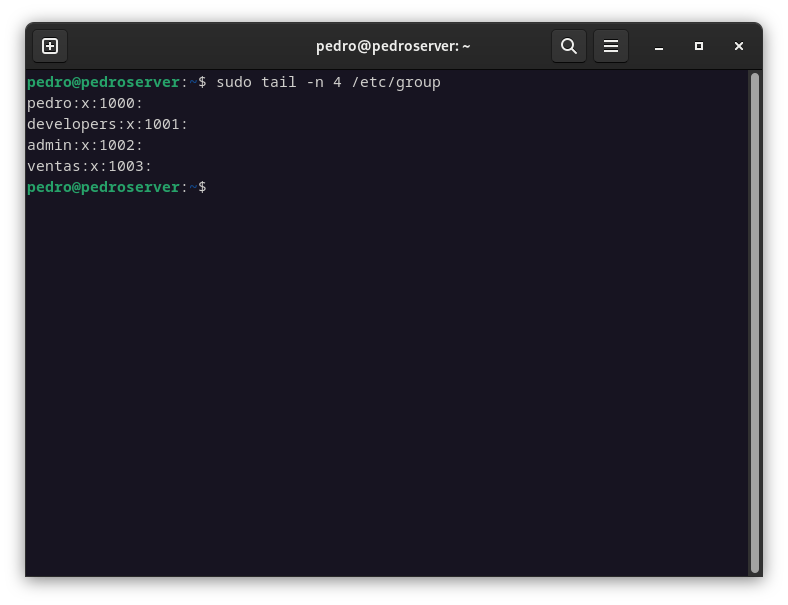
\includegraphics[scale=0.30]{00}
	\caption{Demostración de que los grupos han sido creados}
\end{figure}

\section{Creación de la política de seguridad de contraseñas}

Para la creación de la política de seguridad, necesitamos un móulo adicional de PAM, dicho módulo nos permite que cuando un usuario cambie de contraseña, esta sea comprobada por este módulo se asegura que bajo los parámetros que hemos introducido en un fichero localizado en \textbf{/etc/pam.d/common-password}, se asegure de la longitud y la diferencia de carácteres. Fuente Debian \footnote{https://www.debian.org/doc/manuals/securing-debian-manual/ch04s11.en.html}. Package \footnote{https://packages.debian.org/buster/libpam-cracklib}
\vspace{5mm}

Lo que necesitamos es la siguiente línea, que nos permite cumplir con los siguientes requisitos:

\begin{enumerate}
\item 8 carácteres mínimo.
\item 3 tipos de carácteres diferentes.
\end{enumerate}


\begin{lstlisting}[style=mybash]
sudo apt install libpam-cracklib
sudo nano /etc/pam.d/common-password

# Dentro del fichero introducimos lo siguiente.
password   required     pam_cracklib.so retry=3 minlen=8 difok=3
\end{lstlisting}
    
Enumeración de los parámetros de la línea de parámetros del módulo libpam-cracklib.

\begin{enumerate}
\item retry=3 - Se refiere a los intentos que tiene el usuario de introducir una contraseña buena en passwd.
\item minlen=8 - Se refiere a la cantidad mínima de carácteres que necesita la contraseña.
\item difok=3 - Se especifica el nº mínimo de carácteres que tiene que tener de diferencia con respecto a la contraseña antigua. Por ejemplo: Password -> Password123. Está permitido, pero es una contraseña débil, pero para ello se pueden poner parámetros especiales que incrementen la seguridad como lcredit, ucredit, dcredit, ocredit. Que implican obligar a los usuarios que tengan un crédito negativo, que utilicen una cierta cantidad de carácteres en mayúsculas, números, o carácteres especiales.
\end{enumerate}

Manual de consulta de la información de libpam-cracklib \footnote{https://deer-run.com/users/hal/sysadmin/pam\_cracklib.html}

\begin{figure}[H]
	\centering
	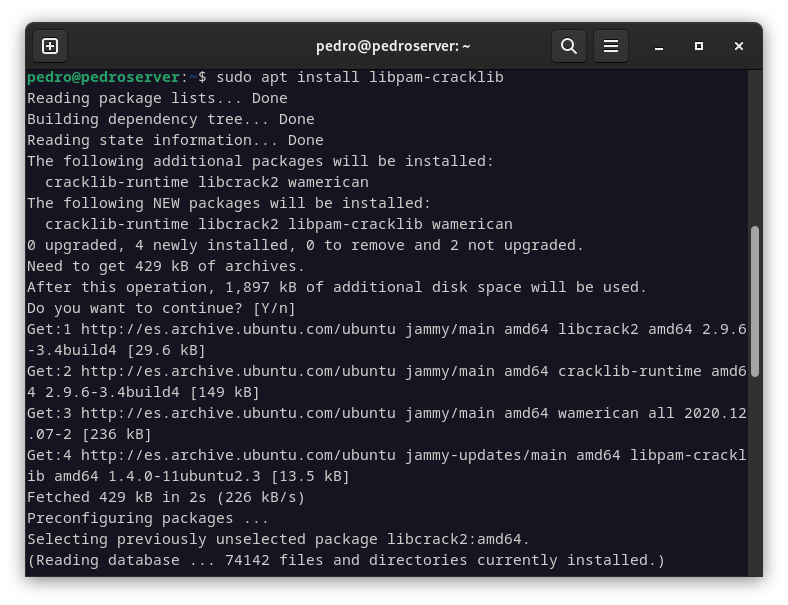
\includegraphics[scale=0.30]{01}
	\caption{Instalación de libpam-cracklib}
\end{figure}

\begin{figure}[H]
	\centering
	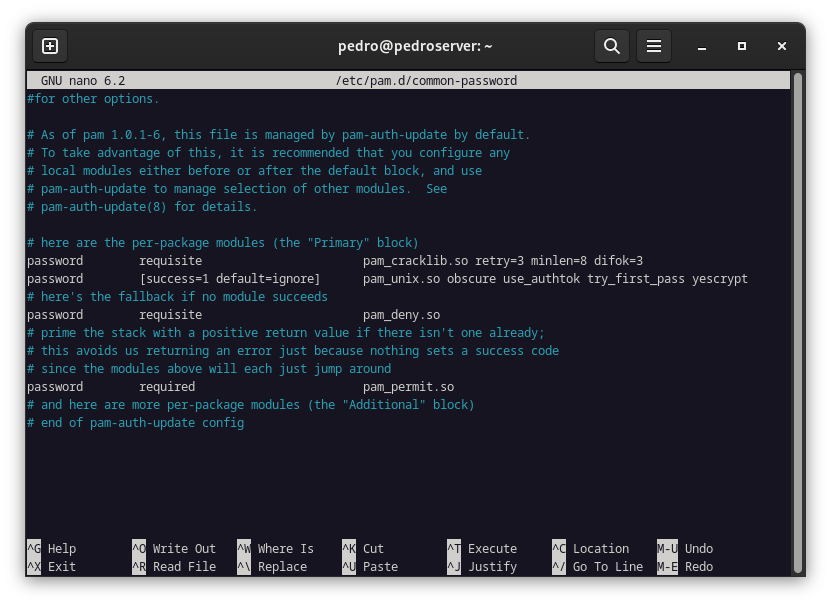
\includegraphics[scale=0.30]{02}
	\caption{Introdución de la línea de libpam-cracklib}
\end{figure}

Si creamos contraseñas muy similares, no nos permitirá hacer nada.

\begin{figure}[H]
	\centering
	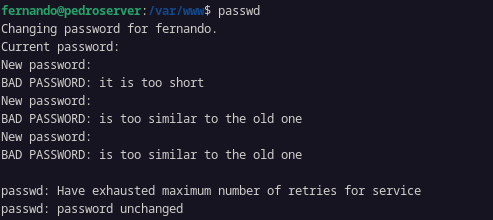
\includegraphics[scale=0.30]{05}
	\caption{Provocando fallos y contraseñas muy similares}
\end{figure}

\newpage
\section{Creación de los usuarios.}

\begin{itemize}
\item Fernando y Pedro2 perteneciente al grupo -> Developers
\item Ivan y Leticia perteneciente al grupo -> Admins
\item Manu y Javi perteneciente al grupo -> Ventas
\end{itemize}
    
Comandos utilizados:

\begin{lstlisting}[style=mybash]
sudo useradd -g developers -e `date -d "1 days" +%Y-%m-%d` -s /bin/bash -m  -k /etc/skel --password `openssl passwd -1 -salt xyz password` fernando ;

sudo useradd -g developers -e `date -d "1 days" +%Y-%m-%d` -s /bin/bash -m  -k /etc/skel --password `openssl passwd -1 -salt xyz password` pedro2 ;

sudo useradd -g admin -e `date -d "1 days" +%Y-%m-%d` -s /bin/bash -m  -k /etc/skel --password `openssl passwd -1 -salt xyz password` ivan ;

sudo useradd -g admin -e `date -d "1 days" +%Y-%m-%d` -s /bin/bash -m  -k /etc/skel --password `openssl passwd -1 -salt xyz  password` leticia ; 

sudo useradd -g ventas -e `date -d "1 days" +%Y-%m-%d` -s /bin/bash -m  -k /etc/skel --password `openssl passwd -1 -salt xyz password` javi ;

sudo useradd -g ventas -e `date -d "1 days" +%Y-%m-%d` -s /bin/bash -m  -k /etc/skel --password `openssl passwd -1 -salt xyz password` manu ;
\end{lstlisting}

El comando utilizado, implica que se cree una caducidad de las cuentas de usuario de un día a partir de su creación. Luego se indica que se crea una contraseña por defecto y se añade a los grupos indicados.

\begin{figure}[H]
	\centering
	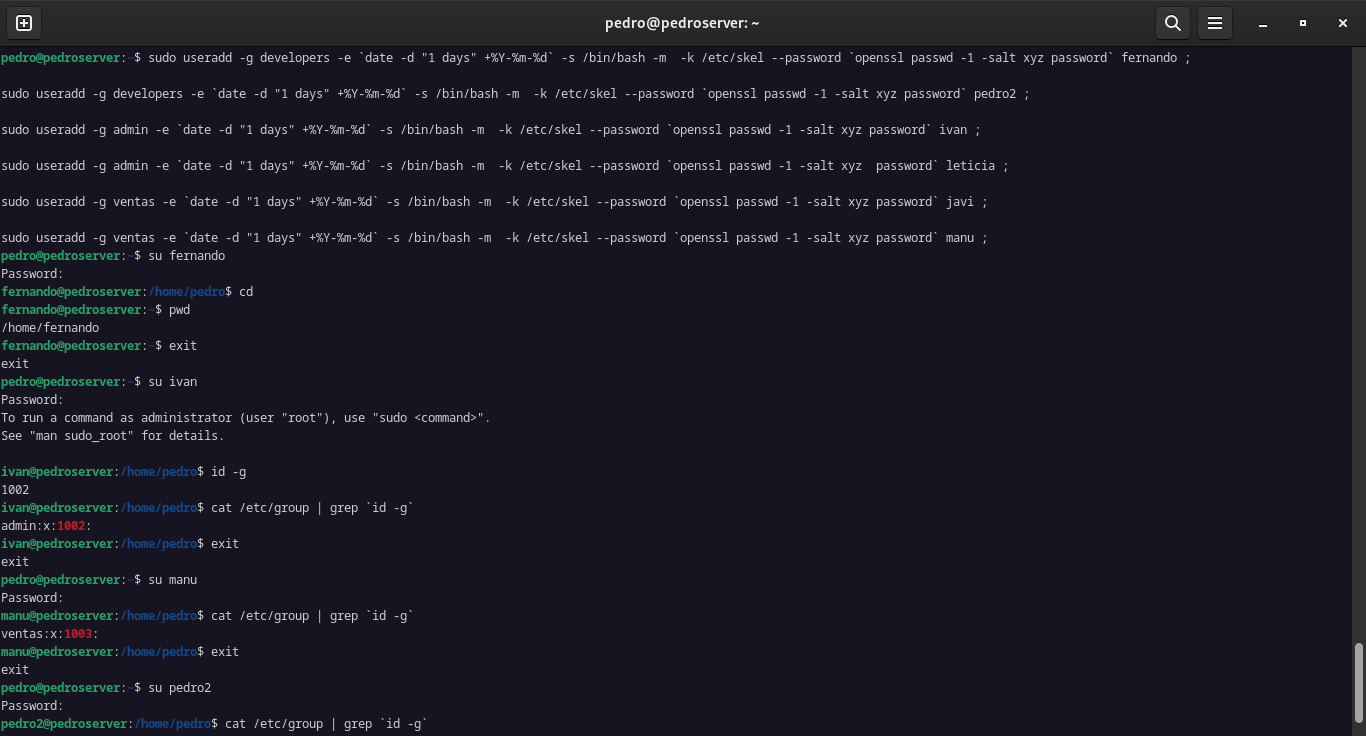
\includegraphics[scale=0.30]{03}
	\caption{Demostración de la creación de usuarios y pruebas de que han sido creados en su grupo}
\end{figure}

\begin{figure}[H]
	\centering
	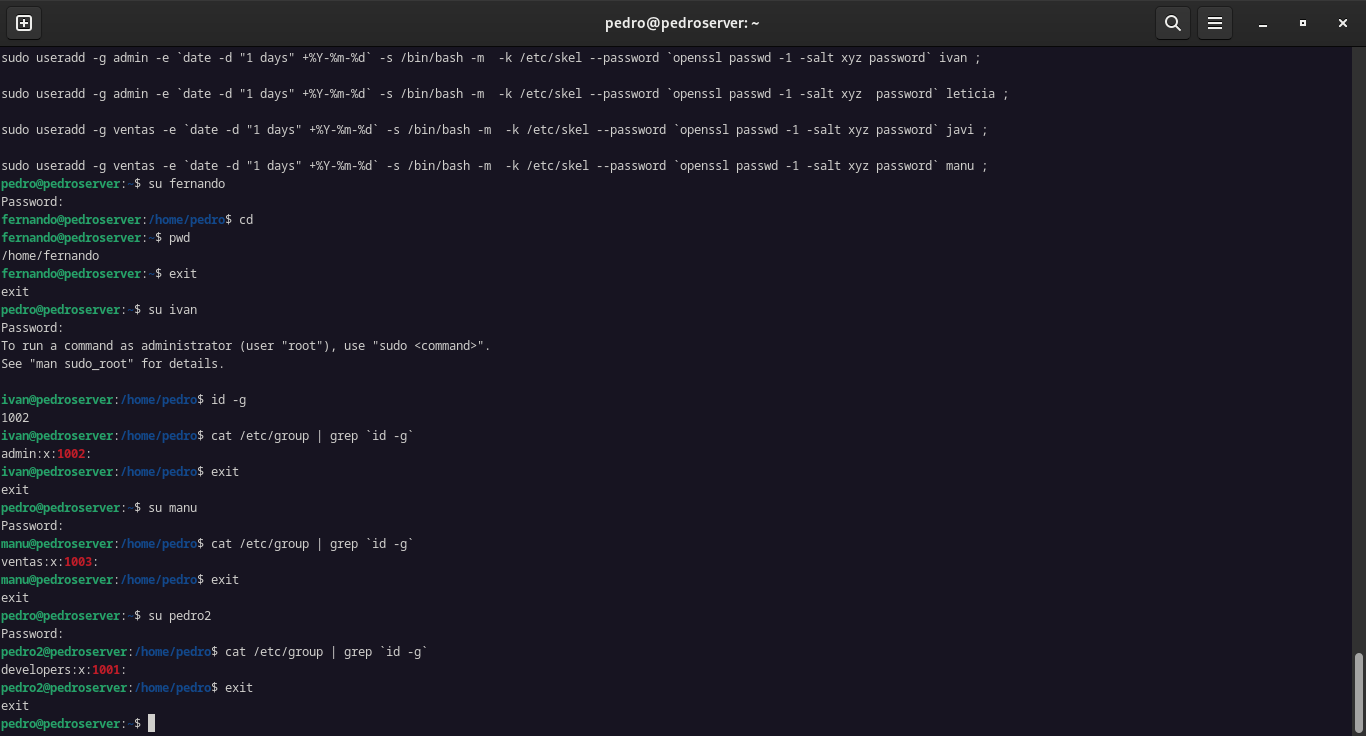
\includegraphics[scale=0.30]{04}
	\caption{Demostración de que la creación de usuarios y pruebas parte 2}
\end{figure}

En las pruebas obtenemos los GID de los grupos a los que pertenece el usuario y los cotejamos con el fichero \textbf{/etc/group}, verificando que se hayan creado con un GID asignado.

\newpage
\section{Creación de los permisos sobre las carpetas}

Utilizamos ACL para la gestión de los permisos sobre las carpetas. Esto es porque si modificamos a nivel de sistema de ficheros, podemos dejar sin acceso a los grupos legítimos o originales el acceso, lectura, escritura y ejecución de los ficheros/directorios.
\vspace{5mm}

Instalamos el paquete de ACL que es necesario.

\begin{lstlisting}[style=mybash]
sudo apt install acl
\end{lstlisting}

Luego el paquete tiene dos herramientas que son muy útiles, una de ver los permisos y los grupos. Otra de asignarlos sobre grupos sin modificar los permisos originales.

\begin{lstlisting}[style=mybash]
sudo mkdir /var/www
sudo mkdir /var/public
# Permisos de developers
sudo setfacl -RPm g:developers:rwx /var/www
sudo setfacl -RPm g:developers:rwx /var/public
sudo setfacl -RPm g:developers:r-- /media

# Permisos de admin
sudo setfacl -RPm g:admin:rwx /

# Permisos de ventas
sudo setfacl -RPm g:ventas:rwx /var/ventas
sudo setfacl -RPm g:ventas:rwx /var/public
\end{lstlisting}

El setfacl de la raíz rompe el sistema, ya que crea conflictos con los archivos del sistema generando que no tengan un comportamiento correcto, lo que no es recomendable utilizar esta parte del ejercicio en el futuro.

Referenecias usadas: \footnote{https://www.redhat.com/sysadmin/linux-access-control-lists} \footnote{https://linux.die.net/man/1/setfacl}

% \begin{lstlisting}[style=mybash]
%     # Para una base de datos concreta
%     mysqldump --user=tiendabd --password=password --databases tiendabd --add-drop-database --add-drop-table [--replace] --host=127.0.0.1 --result-file=dump.sql
% \end{lstlisting}



%\begin{figure}[H]
%	\centering
%	\includegraphics[scale=0.30]{cuestion_1_1}
%	\caption{Se puede ver que al no haber un fallo grave, el sistema lo nota como que sigue funcionando pero en un estado degradado.}
%\end{figure}

%\newpage

%Se pueden hacer include en latex
%\newpage

\section{Section}

\subsection{Subseccion}

\subsubsection{Subseccion}



%-------Bibliografia-----------------------------

%\newpage
\section{Bibliografía}

% Ejemplo
\footnote{Administración de mdadm - Por Red Hat}
\textcolor{blue}{\url{https://access.redhat.com/documentation/en-us/red_hat_enterprise_linux/8/html/managing_storage_devices/managing-raid_managing-storage-devices#monitoring-raid_managing-raid}}



\end{document}
